\chapter{Single Particle Physics}
In this chapter, all units are SI with the exception of temperature,
which is defined in the historical units of eV (electron-volts).\\

\noindent
$e$ is the elementary electric charge\\
$q$ is the total particle charge\\
$Z$ is the particle atomic (proton) number\\
$m$ is the particle mass\\
$\textbf{r}$ is the particle position\\
$\textbf{v}$ is the particle velocity\\
$U$ is energy\\
$T$ is temperature; $T_\mathrm{keV}$ = $T$ in units of kiloelectron-volts\\
$\textbf{E}$ and $\textbf{B}$ are the electric and magnetic fields\\
$\hat{\textbf{b}}$ is a unit vector in the direction of $\textbf{B}$\\
$||$ and $\perp$ indicate parallel and perpendicular to $\hat{\textbf{b}}$\\

\section{Single Particle Motion in \textbf{E} and \textbf{B} Fields}

\subsection{General Formulation}
Single particle trajectories result from solving Newton's second law
for a particle with charge q and mass m in electric and magnetic fields: \scite{freidberg-PP}{141}
\flatwo{
  m\frac{d\textbf{v}}{dt} &= q\left(\textbf{E} + \textbf{v} \times \textbf{B}\right) &
  \frac{d\textbf{r}}{dt} = \textbf{v} 
}{6}

\noindent
If \textbf{E} and \textbf{B} are independent of time, the particle's kinetic and potential
energy is conserved \scite{freidberg-PP}{142}
\fla{ \frac{1}{2}mv^2 + qV &= \textrm{constant} &}
\indent
where $V$ is the scalar potential ($\textbf{E} = -\nabla V$).

\index{Gryo motion in E and B fields}
\subsection{Gyro Motion Solutions for \textbf{B} = B$_0\boldsymbol{\hat{z}}$; \textbf{E} = 0}
Particle initially has $\textbf{r} = (x_0,y_0,z_0), \textbf{v} =
\textbf{v}_\parallel + \textbf{v}_\perp$, and arbitrary phase, $\phi$.\\

\noindent
Parallel to the field: \scite{freidberg-PP}{143}
\fla{ z(t) &= z_0 + v_\parallel t &}
Perpendicular to the field: \scite{freidberg-PP}{144}
\flatwo{
x(t) &= x_g + \rho_L\sin(\Omega_ct - \phi) & x_g &\equiv x_0 + \rho_L\sin\phi \\
y(t) &= y_g + \rho_L\cos(\Omega_ct - \phi) & y_g &\equiv y_0 - \rho_L\cos\phi
}{3}
The guiding center position is ($x_g,y_g$); the larmor (or gyro)
radius is $\rho_L = v_\perp / \Omega_c = mv_\perp / qB$; the
larmor (or gyro) frequency is $\Omega_c$

\index{Single particle drifts}
\index{Radius of curvature}
\subsection{Single Particle Drifts}
In this section, $\mathbf{R}_c$ is the particle's radius of curvature
in a magnetic field and is defined as $\mathbf{b}\cdot\nabla\mathbf{b}
= -\mathbf{R}_c/R_c^2$\\

\index{Drifts! E$\times$B}
\index{E$\times$B drift}
\noindent
E$\times$B drift \scite{freidberg-PP}{149}
\fla{ \textbf{v}_E &= \frac{\textbf{E}\times\textbf{B}}{B^2} &}

\index{Drifts! grad-B}
\index{Grad-B drift}
\noindent
$\nabla$B drift \scite{freidberg-PP}{153}
\noindent
\fla{ \textbf{v}_{\nabla B} &= \frac{mv_\perp^2}{2qB}\frac{\textbf{B} \times \nabla B}{B^2} &}

\index{Drifts! Curvature}
\index{Curvature drift}
\noindent
Curvature drift \scite{freidberg-PP}{159}
\fla{ \textbf{v}_\kappa &= \frac{mv_\parallel^2}{qB}\frac{\boldsymbol{R_c} \times \textbf{B}}{R_c^2B} &}

\index{Drifts! Polarization}
\index{Polarization drift}
\noindent
Polarization drift \scite{freidberg-PP}{162}
\fla{ \textbf{v}_p &= \frac{m}{qB}\boldsymbol{\hat{b}} \times \frac{d\textbf{v}_E}{dt} &}

\noindent
Vacuum field only $\rightarrow \nabla \times \textbf{B}=0$ \scite{freidberg-PP}{160}
\fla{ \textbf{v}_{\nabla B} + \textbf{v}_\kappa &= \frac{m}{qB}(v_\parallel^2 + \frac{v_\perp^2}{2})\frac{\boldsymbol{R_c} \times \textbf{B}}{R_c^2B} &}

\noindent
Particle drift velocity for a general force $\mathbf{F}$ \scite{freidberg-PP}{153}
\fla{ \textbf{v}_F &= \frac{\textbf{F}\times\textbf{B}}{qB^2} &}


\index{Magnetic mirroring}
\index{Magnetic moment}
\subsection{Magnetic Moment And Mirroring} 
In this section, $i$ refers to the initial point, and $f$ stand for
the final, or mirror, point.\\  

\index{First adiabatic invariant}
\noindent
Magnetic moment (the first adiabatic invariant) \scite{freidberg-PP}{167}
\fla{ \mu &= \frac{mv_\perp^2(t)}{2B(t)} = \mathrm{constant} &} 
Force on particle in magnetic fields where $\nabla B/B \ll 1$ \scite{freidberg-PP}{171}
\fla{ F_\parallel &\approx -\mu\nabla_\parallel B &} 
Velocity in terms of velocity space pitch angle \scite{freidberg-PP}{174}
\flatwo{ v_{\perp i} &= v_0\sin\theta & v_{\parallel i} = v_0\cos\theta}{7}
Conservation of energy \scite{freidberg-PP}{174}
\fla{ \frac{1}{2} m\left(v_{\perp i}^2 + v_{\parallel i}^2 \right) &= \frac{1}{2}mv_{\perp f}^2 = U_\mathrm{total} = \mathrm{constant} &}

\index{Mirroring condition} 
\noindent
Mirroring condition \scite{freidberg-PP}{175}
\fla{ \sin^2\theta_c&= \frac{U_{\perp i}}{U_\mathrm{total}} = \frac{v_{\perp i}^2}{v_{\perp f}^2} = \frac{B_{min}}{B_{max}} &} 

\index{Trapped particle fraction} 
\noindent
Fraction of trapped particles (Maxwellian distribution) \scite{freidberg-PP}{176}
\fla{ \mathcal{F}_{\mathrm{trapped}} &= \frac{1}{n}\int_{\theta_c}^{\pi-\theta_c}\sin\theta d\theta \int_0^{2\pi} d \phi \int_0^\infty \mathcal{F}_{\mathrm{Maxwellian}}(v) v^2 dv &}
where $n$ is the total number of particles in the distrubition function


\index{Binary coulomb collisions}
\section{Binary Coulomb Collisions}

\noindent r is the relative distance\\
\textbf{v}$_1$ and \textbf{v}$_2$ are particle velocities in the lab
frame\\
\textbf{V} and \textbf{v} are the center of mass and relative
velocities\\
v$_0$ and b$_0$ are the initial relative velocity and impact parameter\\
$\chi$ is the scattering angle in the center of mass frame\\
$\dot{x}$ is the time derivative of quantity x\\

\begin{figure}[h!]
  \centering
  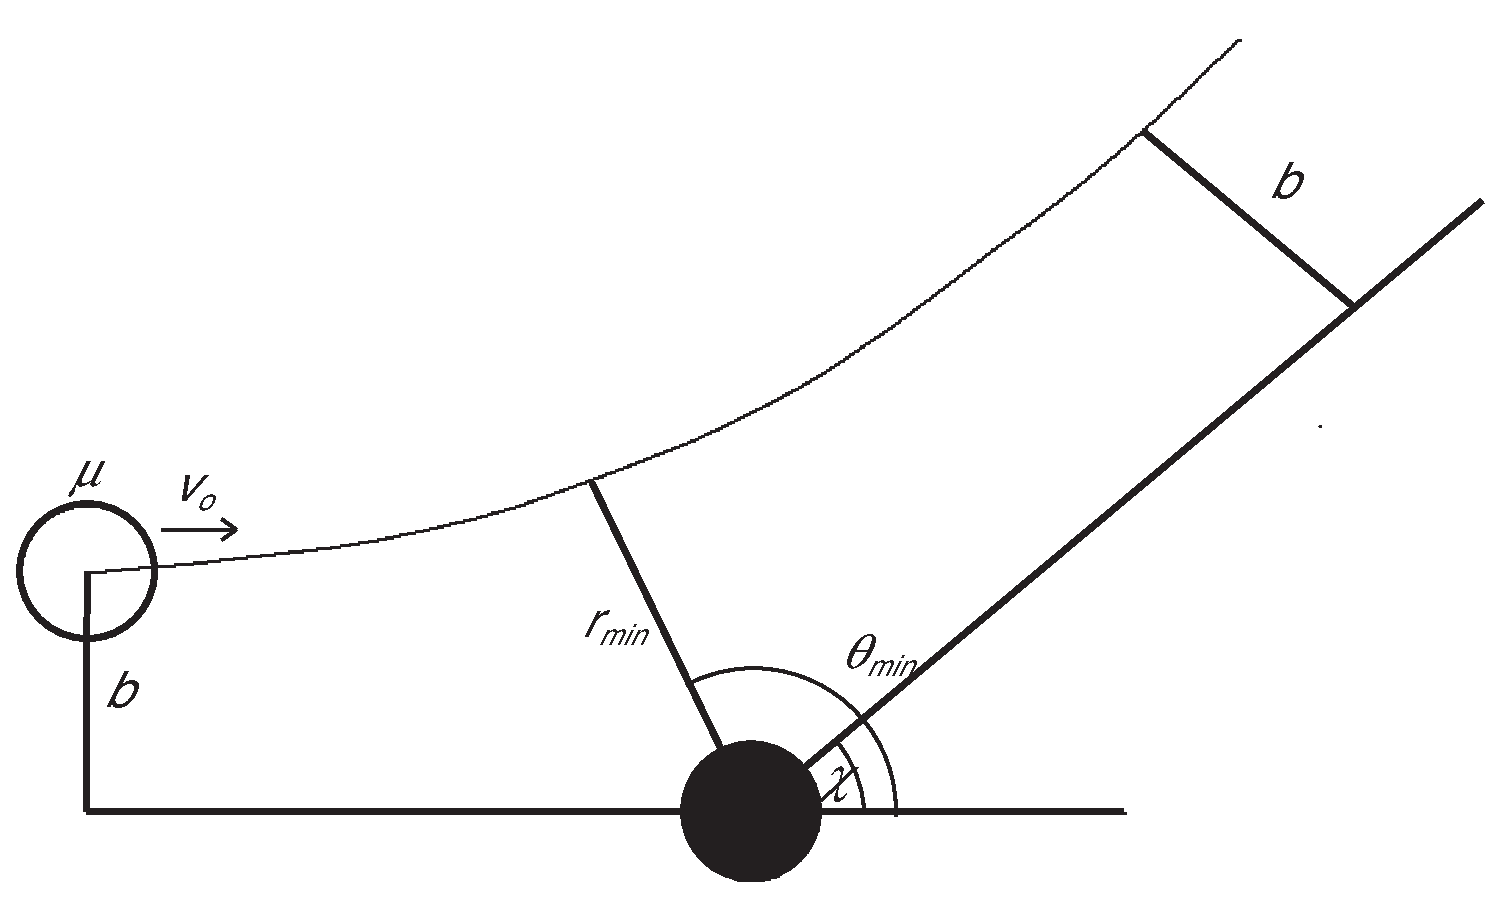
\includegraphics[width = 0.7\textwidth]{figures/twoBodyCollision.eps}
  \caption*{Schematic of two body collision in the reduced mass frame.}
  \label{fig:2body_collision}
\end{figure}

\noindent
Force between 2 charged particles
\fla{ \textbf{F} &= -\nabla\left(\frac{q_1q_2}{4\pi\epsilon_0r}\right) &}
\index{Center of mass transformation}
\noindent
Transformation to center of mass frame \scite{freidberg-PP}{186}
\flatwo{
  \textbf{V} &= \frac{m_1\textbf{v}_1 + m_2\textbf{v}_2}{m_1 + m_2} &\textbf{v} &= \textbf{v}_1 - \textbf{v}_2 \\
  \textbf{v}_1 &= \textbf{V} + \frac{m_2\textbf{v}}{m_1+m_2} & \textbf{v}_2 &= \textbf{V} - \frac{m_1\textbf{v}}{m_1+m_2}
}{3}
\index{Reduced mass}
\noindent
Reduced mass \scite{freidberg-PP}{186}
\fla{ m_\mu &= \frac{m_1m_2}{m_1+m_2} &}
Conservation of energy \scite{freidberg-PP}{187}
\fla{ \frac{1}{2}m_\mu v^2 + \frac{q_1q_2}{4\pi\epsilon_0r} &= E_0 = \frac{1}{2}m_\mu v^2_0 = \mathrm{constant} &}
Conservation of angular momentum \scite{freidberg-PP}{187}
\fla{ m_\mu \textbf{r} \times \textbf{v} &= \textbf{L}_0 = -m_\mu bv_0 = \mathrm{constant} &}
Transformation to cylindrical coordinates \scite{freidberg-PP}{188}
\flatwo{ \textbf{r} &= r\boldsymbol{\hat{r}} & \textbf{v} = \dot{r}\boldsymbol{\hat{r}}+r\dot{\theta}\boldsymbol{\hat{\theta}}}{8}
Ordinary differential equation for unknown r(t) \scite{freidberg-PP}{188}
\fla{ \dot{r} &=\mp v_0\left(1 - 2\frac{b_{90}}{r} - \frac{b^2}{r^2}\right)^{1/2} &}
Solution in terms of scattering angle $\chi$ \scite{freidberg-PP}{190}
\fla{ \tan(\frac{\chi}{2}) &= \frac{b_{90}}{b} = \frac{q_1q_2}{4\pi\epsilon_0 m_\mu v_0^2 b} &}
Impact parameter for 90 degree collision \scite{freidberg-PP}{188}
\fla{ b_{90} &= \frac{q_1q_2}{4\pi \epsilon_0 m_\mu v_0^2} &}

\section{Single Particle Collisions with Plasma}
$a$ is an approaching test particle; $t$ is a target plasma particle.
$Q_\mathrm{at}$ are quantities depending on approaching particle $a$
incident upon target particle $t$.\\

\noindent
Total loss in test particle linear momentum \scite{freidberg-PP}{192}
\fla{\frac{d}{dt}(m_av_a) &= -(\Delta m_a v_a)n_t\sigma v_a\\
  &= -\int(\Delta m_a v_a)f_a(\textbf{v}_t)|\textbf{v}_a - \textbf{v}_t|b\,db\,d\alpha\, d^3v &}

\index{Collision frequencies! Definition}
\noindent
Definition of test particle collision frequency \scite{freidberg-PP}{193}
\fla{ \frac{d}{dt}(m_a v_a) &\equiv -\nu_{at}(m_a v_a) &}

\index{Collision frequencies! Evaluation}
\noindent
Test particle collision frequency \scite{freidberg-PP}{193}
\fla{ \nu_{at}(v_a) &= \frac{1}{m_av_a}\int(\Delta m_a v_a)f_t(\textbf{v}_t)|\textbf{v}_a - \textbf{v}_t|b\,db\,d\alpha\,d^3v &}

\subsection{Collision Frequencies}
Approximated expressions for frequencies hold only for $v_{e}\sim v_{te}\gg v_{ti}$\\

\index{Electron-ion collision frequency}
\noindent
Electron-ion \scite{freidberg-PP}{197}
\fla{
  \nu_{ei} &= \left(\frac{e^4n_i \ln\Lambda}{4\pi\epsilon_0^2 m_e m_\mu}\right)\frac{1}{v_e^3 + 1.3v_{ti}^3} \approx \frac{e^4n_i \ln\Lambda}{4\pi\epsilon_0^2 m_e^2 v_e^3} &\\
  &\approx 8.06\times10^5 \frac{n_i \ln\Lambda}{v_e^3} \hspace{0.5cm} [s^{-1}] &
} 

\index{Electron-electron collision frequency}
\noindent
Electron-electron  \scite{freidberg-PP}{197}
\fla{
  \nu_{ee} &= \left(\frac{e^4n_e \ln\Lambda}{2\pi\epsilon_0^2 m_e^2}\right)\frac{1}{v_e^3 + 1.3v_{te}^3} \hspace{0.5cm} [s^{-1}] &
}

\index{Ion-ion collision frequency}
\noindent
Ion-ion  \scite{freidberg-PP}{197}
\fla{
  \nu_{ii} &= \left(\frac{e^4n_i \ln\Lambda}{2\pi\epsilon_0^2 m_i^2}\right)\frac{1}{v_i^3 + 1.3v_{ti}^3} \hspace{0.5cm} [s^{-1}] &
}

\index{Ion-electron collision frequency}
\noindent
Ion-electron \scite{freidberg-PP}{197}
\fla{
  \nu_{ie} &= \left(\frac{e^4n_e \ln\Lambda}{4\pi\epsilon_0^2 m_e m_i}\right)\frac{1}{v_i^3 + 1.3v_{te}^3} \hspace{0.5cm} [s^{-1}] &
}


\index{Collision frequency scalings}
\noindent
Collision frequency scalings \scite{freidberg-PP}{197}
\fla{ \nu_{ee} &\sim \nu_{ei} & \nu_{ii} &\sim \left(\frac{m_e}{m_i}\right)^{1/2}\nu_{ei} & \nu_{ie} &\sim \left(\frac{m_e}{m_i}\right)\nu_{ei}}

\index{Coulomb logarithm}
\noindent
The Coulomb logarithm \scite{freidberg-PP}{194}
\fla{\Lambda & \approx \frac{12 \pi \epsilon_{0}^{3/2} T_{e}^{3/2}}{n_{e}^{1/2}e^3} = 4.9 \times 10^{7} \frac{T_{\textrm{kev}}^{3/2}}{n_{20}^{1/2}} &}

where $\ln \Lambda \approx 15-20$ for most plasmas.


\subsection{Collision Times}

\index{Electron collision time}
\index{Times! electron collision}
\noindent
Electron-ion collision time \scite{helander}{5} %Helander Sigmar p5
\fla{ \tau_{ei} &= \frac{12\pi^{3/2}\epsilon_0^2m_e^{1/2}T_e^{3/2}}{\sqrt{2}n_iZ_i^2e^4\ln\Lambda} &\\
  &= 1.09\times10^{16}\frac{T_\mathrm{e,~keV}^{3/2}}{Z_i^2n_{i}\ln\Lambda} \hspace{0.5cm} [s] &}

\index{Times! ion collision}
\index{Ion collision time}
\noindent
Ion-ion collision time \scite{helander}{5}% Helander Sigmar p5; note factor in \tau_i was 6.6\times 10^17
\fla{ \tau_{ii} &= \frac{12\pi^{3/2}}{2^{1/2}}\frac{ \epsilon_0^2m_i^{1/2}T_i^{3/2}}{n_iZ_{i}^4e^4\ln\Lambda_i} &\\
  &= 4.67\times10^{17}\left(\frac{m_i}{m_p}\right)^{1/2}\frac{T_\mathrm{i,~keV}^{3/2}}{Z_i^4n_{i}\ln\Lambda_i} \hspace{0.5cm} [s] &}

An ion collision time is sometimes defined to be $\tau_{i}=\sqrt{2}\tau_{ii}$

\index{Times! ion-impurity collision}
\index{Ion-impurity collision time}
\noindent Ion-impurity collision time \scite{helander}{177} % Helander Sigmar pp177
\fla{
  \tau_{iI} &= \frac{12 \pi^{3/2}}{2^{1/2}} \frac{m_{i}^{1/2} T_{i}^{3/2} \epsilon_{0}^{2}}{n_{I}Z_{i}^{2} Z_{I}^{2} e^{4} \ln \Lambda} &\\
           &=  4.67\times10^{17}\left(\frac{m_i}{m_p}\right)^{1/2}\frac{T_\mathrm{i,~keV}^{3/2}}{Z_i^2Z_{I}^2n\ln\Lambda_i} \hspace{0.5cm} [s] &
}
\index{Energy transfer time}
\index{Times! energy tranfer}
\noindent
Electron-to-ion energy transfer time %Where is this from?
\fla{ R_\mathrm{ei} &= \frac{\frac{3}{2}n\left(T_e - T_i\right)}{\left(\frac{m_i}{2m_e}\tau_e\right)} &}

\index{Thermal equilibration}
\noindent
Thermal equilibration frequency (rate of species a equilibrating to species b) \scite{huda}{34}\\
\fla{\nu_{ab}^{t}  &= 1.8 \times 10^{-19} \frac{ (m_{a}m_{b})^{1/2} Z_{a}^{2}Z_{b}^{2} n_{b} \ln \Lambda}{(m_{a}T_{b}+ m_{b}T_{a})^{3/2}} \hspace{0.5cm} \mathrm{[s^{-1}]} &}

\indent For ions and electrons with $T_{e}\approx T_{i}=T$, $\nu_{ei}n_{e}=\nu_{ie}n_{i}$ \scite{huda}{34}\\
\fla{\nu^{t}_{ei} &= 3.2 \times 10^{-15} \frac{Z^{2} \ln \Lambda}{(m_{i}/m_{p} T^{3/2})} \hspace{0.5cm} \mathrm{[m^{3}s^{-1}]} &}


\section{Particle Beam Collisions with Plasmas}
In this section, plasma density is written as $n_{20}$ = $n/10^{20}$\\

\index{Beam-electron collision frequency}
\noindent
Beam-electron collision frequency \scite{freidberg-PP}{202-203}
\fla{
  \nu_{be}(v_b) &= \left(\frac{Z_b^2e^4n_e\ln\Lambda}{4\pi\epsilon_0^2 m_e m_b}\right)\frac{1}{v_b^3 + 1.3v_{te}^3} &\\
  &\approx \frac{1}{3(2\pi)^{3/2}}\frac{Z_b^2e^4m_e^{1/2}n_e\ln\Lambda}{\epsilon_0^2m_bT_e^{3/2}} \hspace{.5cm} \text{($v_{te}^3 \gg v_b^3$ only)}&\\
  &= 100\frac{n_{20}}{T_{\textrm{keV}}^{3/2}} \hspace{0.5cm} \textrm{[s$^{-1}$]} \hspace{0.5cm} \textrm{(alpha heating only)} &
}

\index{Beam-ion collision frequency}
\noindent
Beam-ion collision frequency \scite{freidberg-PP}{203}
\fla{
  \nu_{bi}(v_b) & = \left(\frac{Z_b^2e^4n_i\ln\Lambda}{4\pi\epsilon_0^2m_\mu m_b}\right)\frac{1}{v_b^3 + 1.3v_{ti}^3} &\\
  &\approx \frac{1}{4\pi}\frac{Z_b^2e^4n_i\ln\Lambda}{\epsilon_0^2m_\mu m_b v_b^3} \hspace{.5cm} \text{($v_{ti}^3 \ll v_b^3$ only)}&\\
  &= 0.94\frac{n_{20}}{(E_{\textrm{beam}})_{\textrm{MeV}}^{3/2}} \hspace{0.5cm} \textrm{[s$^{-1}$]} \hspace{0.5cm} \textrm{(alpha heating only)} &
}

\hangindent=0.25 in When $\nu_{be} = \nu_{bi}$, $v_b = v_{crit}$ and
the beam changes the plasma particle it preferentially damps upon.
For $v_b > v_{crit}$, the beam damps on plasma electrons; for $v_b <
v_{crit}$, the beam damps on plasma ions.  The critical beam energy is
calculated as $E_{c}=1/2m_{beam} v_{beam}^2=14.8
(m_{beam}/m_{i}^{2/3})T_{e}$. For a 15 keV plasma, the critical energy
  corresponds to 660 keV.\\


\index{Neutral beam energy loss}
%Wesson p 249
\noindent A high energy beam entering a plasma has energy behavior (purely slowing down on electrons) \scite{wesson}{249}
%\fla{\frac{dE_{beam}/dt &= -\frac{2}{\tau_{se}} E_{beam} \left( 1+E_{c}/E_{beam} \right) &}

\fla{E_{b} &= E_{b,0} \left[ e^{-3t/\tau_{se}} - \left(\frac{E_{c}}{E_{b,0}} \right)^{3/2} \left( 1-e^{-3t/\tau_{se}} \right) \right]^{2/3} &}

\noindent where $E_{b,0}$ is the initial beam energy and $\tau_{se}$ is the slowing down time assuming $v_b < v_{te}$ \scite{wesson}{246}

\fla{ \tau_{se} &=\frac{3 (2\pi)^{3/2} \epsilon_{0}^{2}m_{b}T_{e}^{3/2}}{m_{e}^{1/2}n e^{4} \ln \Lambda}  &}

%\index{Neutral particle beams}
%\subsection{Neutral Particle Beams}
%For a hydrogenic neutral beam ($H_0$) injected into a plamsa, two atomic
%processes dominate the interaction: charge exchange (CX), 
%$H_0 + H^+ \Rightarrow H^+ + H_0$, and impact ionization (II), $H_0 + H^+ \Rightarrow 2H^+ + e^-$
%
%\noindent
%Change in beam flux per unit length
%\fla{ \frac{I_{beam}}{dl} &\approx n_{plasma}(\sigma_{CX} + \sigma_{II})I_{beam} &}
%
%\noindent
%Neutral penetration length
%\fla{ \lambda_{neutral} &= \frac{(5\times10^{17}) E^{beam}_{keV}}{m_{beam}n_{plasma}Z_{effective}} \text{   [m]} &}
%
